% !TeX program = xelatex
% !TeX options = -shell-escape
% !TEX encoding = UTF-8

% --------------------------------------------------------------
% This is all preamble stuff that you don't have to worry about.
% Head down to where it says "Start here"
% --------------------------------------------------------------

\documentclass[12pt]{article}
\usepackage[margin=2cm]{geometry} % 頁面邊距設置
\usepackage{amsmath,amssymb,amsthm} % 數學相關套件
\usepackage{graphicx} % 圖形插入
\usepackage{booktabs} % 表格線條
\usepackage[AutoFakeBold,AutoFakeSlant]{xeCJK} % 中文支援
\usepackage{fancyhdr} % 頁首頁尾設置
\usepackage{xcolor,changepage,mdframed} % 顏色與框線相關
\usepackage{titlesec} % 標題格式
\usepackage{setspace} % 行距
\usepackage{minted} % 程式碼高亮（需安裝 Python 套件 pygments）
\usepackage[shortlabels]{enumitem} % 列表格式
\usepackage[colorlinks=true,linkcolor=black,urlcolor=blue,citecolor=blue]{hyperref}
% 超連結
\graphicspath{{images}}

% 字體設定 (xeCJK)
\setCJKmainfont{黑體-繁}
\setCJKmonofont{Noto Sans CJK TC}

% 頁首/頁尾設定 (fancyhdr)
\pagestyle{fancy}
\fancyhead[L]{NASA Homework 5} % 可以用 \leftmark 取代
\fancyhead[R]{B13901011 吳亞倫}
\fancyfoot[C]{\thepage}
\renewcommand{\headrulewidth}{0.4pt}
\renewcommand{\footrulewidth}{0pt}
\setlength{\headheight}{15pt}

% tex-fmt: off
\newtheorem*{theorem}{Theorem}
\newenvironment{lemma}[2][Lemma]{\begin{trivlist}
\item[\hskip \labelsep {\bfseries #1}\hskip \labelsep {\bfseries #2.}]}{\end{trivlist}}
\newenvironment{exercise}[2][Exercise]{\begin{trivlist}
\item[\hskip \labelsep {\bfseries #1}\hskip \labelsep {\bfseries #2.}]}{\end{trivlist}}
\newenvironment{problem}[2][Problem]{\begin{trivlist}
\item[\hskip \labelsep {\bfseries #1}\hskip \labelsep {\bfseries #2}]}{\end{trivlist}}
\newenvironment{question}[2][Question]{\begin{trivlist}
\item[\hskip \labelsep {\bfseries #1}\hskip \labelsep {\bfseries #2.}]}{\end{trivlist}}
\newenvironment{corollary}[2][Corollary]{\begin{trivlist}
\item[\hskip \labelsep {\bfseries #1}\hskip \labelsep {\bfseries #2.}]}{\end{trivlist}}
\newenvironment{solution}{\begin{proof}[Solution]}{\end{proof}}
\newenvironment{answer}{\begin{proof}[Ans]}{\end{proof}}

% 樣式設定

\setminted{frame=lines, linenos, framesep=2mm, breaklines=true, breakanywhere=true, autogobble=true}

% 自訂框線環境
\newmdenv[
  linewidth=2pt, linecolor=gray, backgroundcolor=gray!10,
  topline=false, bottomline=false, rightline=false,
  skipabove=10pt, skipbelow=10pt, innerleftmargin=10pt,
  innerrightmargin=0pt, innertopmargin=5pt, innerbottommargin=5pt
]{myquote}

\newenvironment{mycolorbox}[1][gray]{
  \renewmdenv[
    linewidth=2pt, linecolor=#1, backgroundcolor=#1!10,
    topline=false, bottomline=false, rightline=false,
    skipabove=10pt, skipbelow=10pt, innerleftmargin=10pt,
    innerrightmargin=0pt, innertopmargin=5pt, innerbottommargin=5pt
  ]{myquote}
  \begin{myquote}
}{\end{myquote}}

\linespread{1.1}
% \usemintedstyle{xcode}
\AtBeginEnvironment{minted}{\vspace{-10pt}} % 可根據需求調整間距數值
\setminted{breaklines=true, breakanywhere=true, autogobble=true}

% tex-fmt: on
\begin{document}
\thispagestyle{fancy}

%------------------------------------------------------------
%                         Start here
% -----------------------------------------------------------

\begin{center}
  {\large \bfseries Network Administration / System Administration} \\
  \vspace{1em}
  {\Large \bfseries Homework 5} \\
\end{center}

\vspace{2em}

\begin{tabular}{@{}l l}
  \textbf{Student:} & 吳亞倫 \\
  \textbf{ID:} & B13901011  \\
  \textbf{Department:} & 電機工程學系
\end{tabular}
\bigskip

\begin{mycolorbox}[cyan]
  \textbf{Discussion Partners:}
  \begin{itemize}
    \item Classmates：賴泓安、鄭竣陽、喻慈恩
      \vspace{0.5em}
  \end{itemize}
\end{mycolorbox}

% ------------------------------------------------------------
%    Problem 1
% ------------------------------------------------------------
\section{Setting up PowerDNS}

% Problem 1-1
\subsection{Install Debian and PowerDNS}
\begin{mycolorbox}[teal]
  \textbf{Reference:} 
  \footnotesize
  \begin{itemize}
    \item \url{https://wiki.debian.org/QEMU}
    \item \href{https://www.cloudpanel.io/tutorial/how-to-add-user-to-sudoers-in-debian/}{How to add user to sudoers in Debian}
    \item \href{https://www.reddit.com/r/linuxquestions/comments/pcfjo6/bash_usermod_command_not_found_in_latest_debian/}{Bash: usermod command not found in latest Debian}
    \item \href{https://computingforgeeks.com/install-powerdns-and-powerdns-admin-on-debian/}{Install PowerDNS and PowerDNS Admin on Debian}
    \item \url{https://repo.powerdns.com/}
    \item \url{https://doc.powerdns.com/authoritative/installation.html}
    \item \href{https://wiki.freedomstu.com/books/%E9%96%8B%E6%BA%90%E8%BB%9F%E9%AB%94%E5%AE%89%E8%A3%9D%E6%B5%81%E7%A8%8B/page/powerdns-debian}{PowerDNS 架設 - Debian}
  \end{itemize}
\end{mycolorbox}
\begin{enumerate}
  \item 我連線到工作站上，並且下載 Debian 12.10.0 的 \href{https://cdimage.debian.org/debian-cd/current/amd64/iso-cd/debian-12.10.0-amd64-netinst.iso}{netinst.iso} 安裝檔案。
  \item 使用 \texttt{qemu-img} 建立一個 16GB 的 qcow2 磁碟檔案。
  \begin{minted}{bash}
    qemu-img create -f qcow2 debian.qcow 16G
  \end{minted}
  \item 使用 \texttt{qemu-system-x86\_64} 開啟虛擬機器。連線到 port 7000 後，安裝 Debian 12。
  \begin{minted}{bash}
    qemu-system-x86_64 \
      -enable-kvm \
      -m 2048 \
      -smp 2 \
      -cpu host \
      -cdrom debian-12.10.0-amd64-netinst.iso \
      -drive file=debian.qcow2 \
      -boot d \
      -net nic -net user \
      -vnc :1100
  \end{minted}
  \item 在安裝精靈當中，我設定 Hostname 為 \texttt{debian}，User name、Root password 以及 User password 為我的學號，Debian Archive Mirror 為 \texttt{debian.csie.ntu.edu.tw}，並且選擇安裝 gnome desktop、SSH server 和 Standard system utilities。其餘選項以及 Grub 設定我都使用預設值。
  \begin{figure}[H]
    \centering
    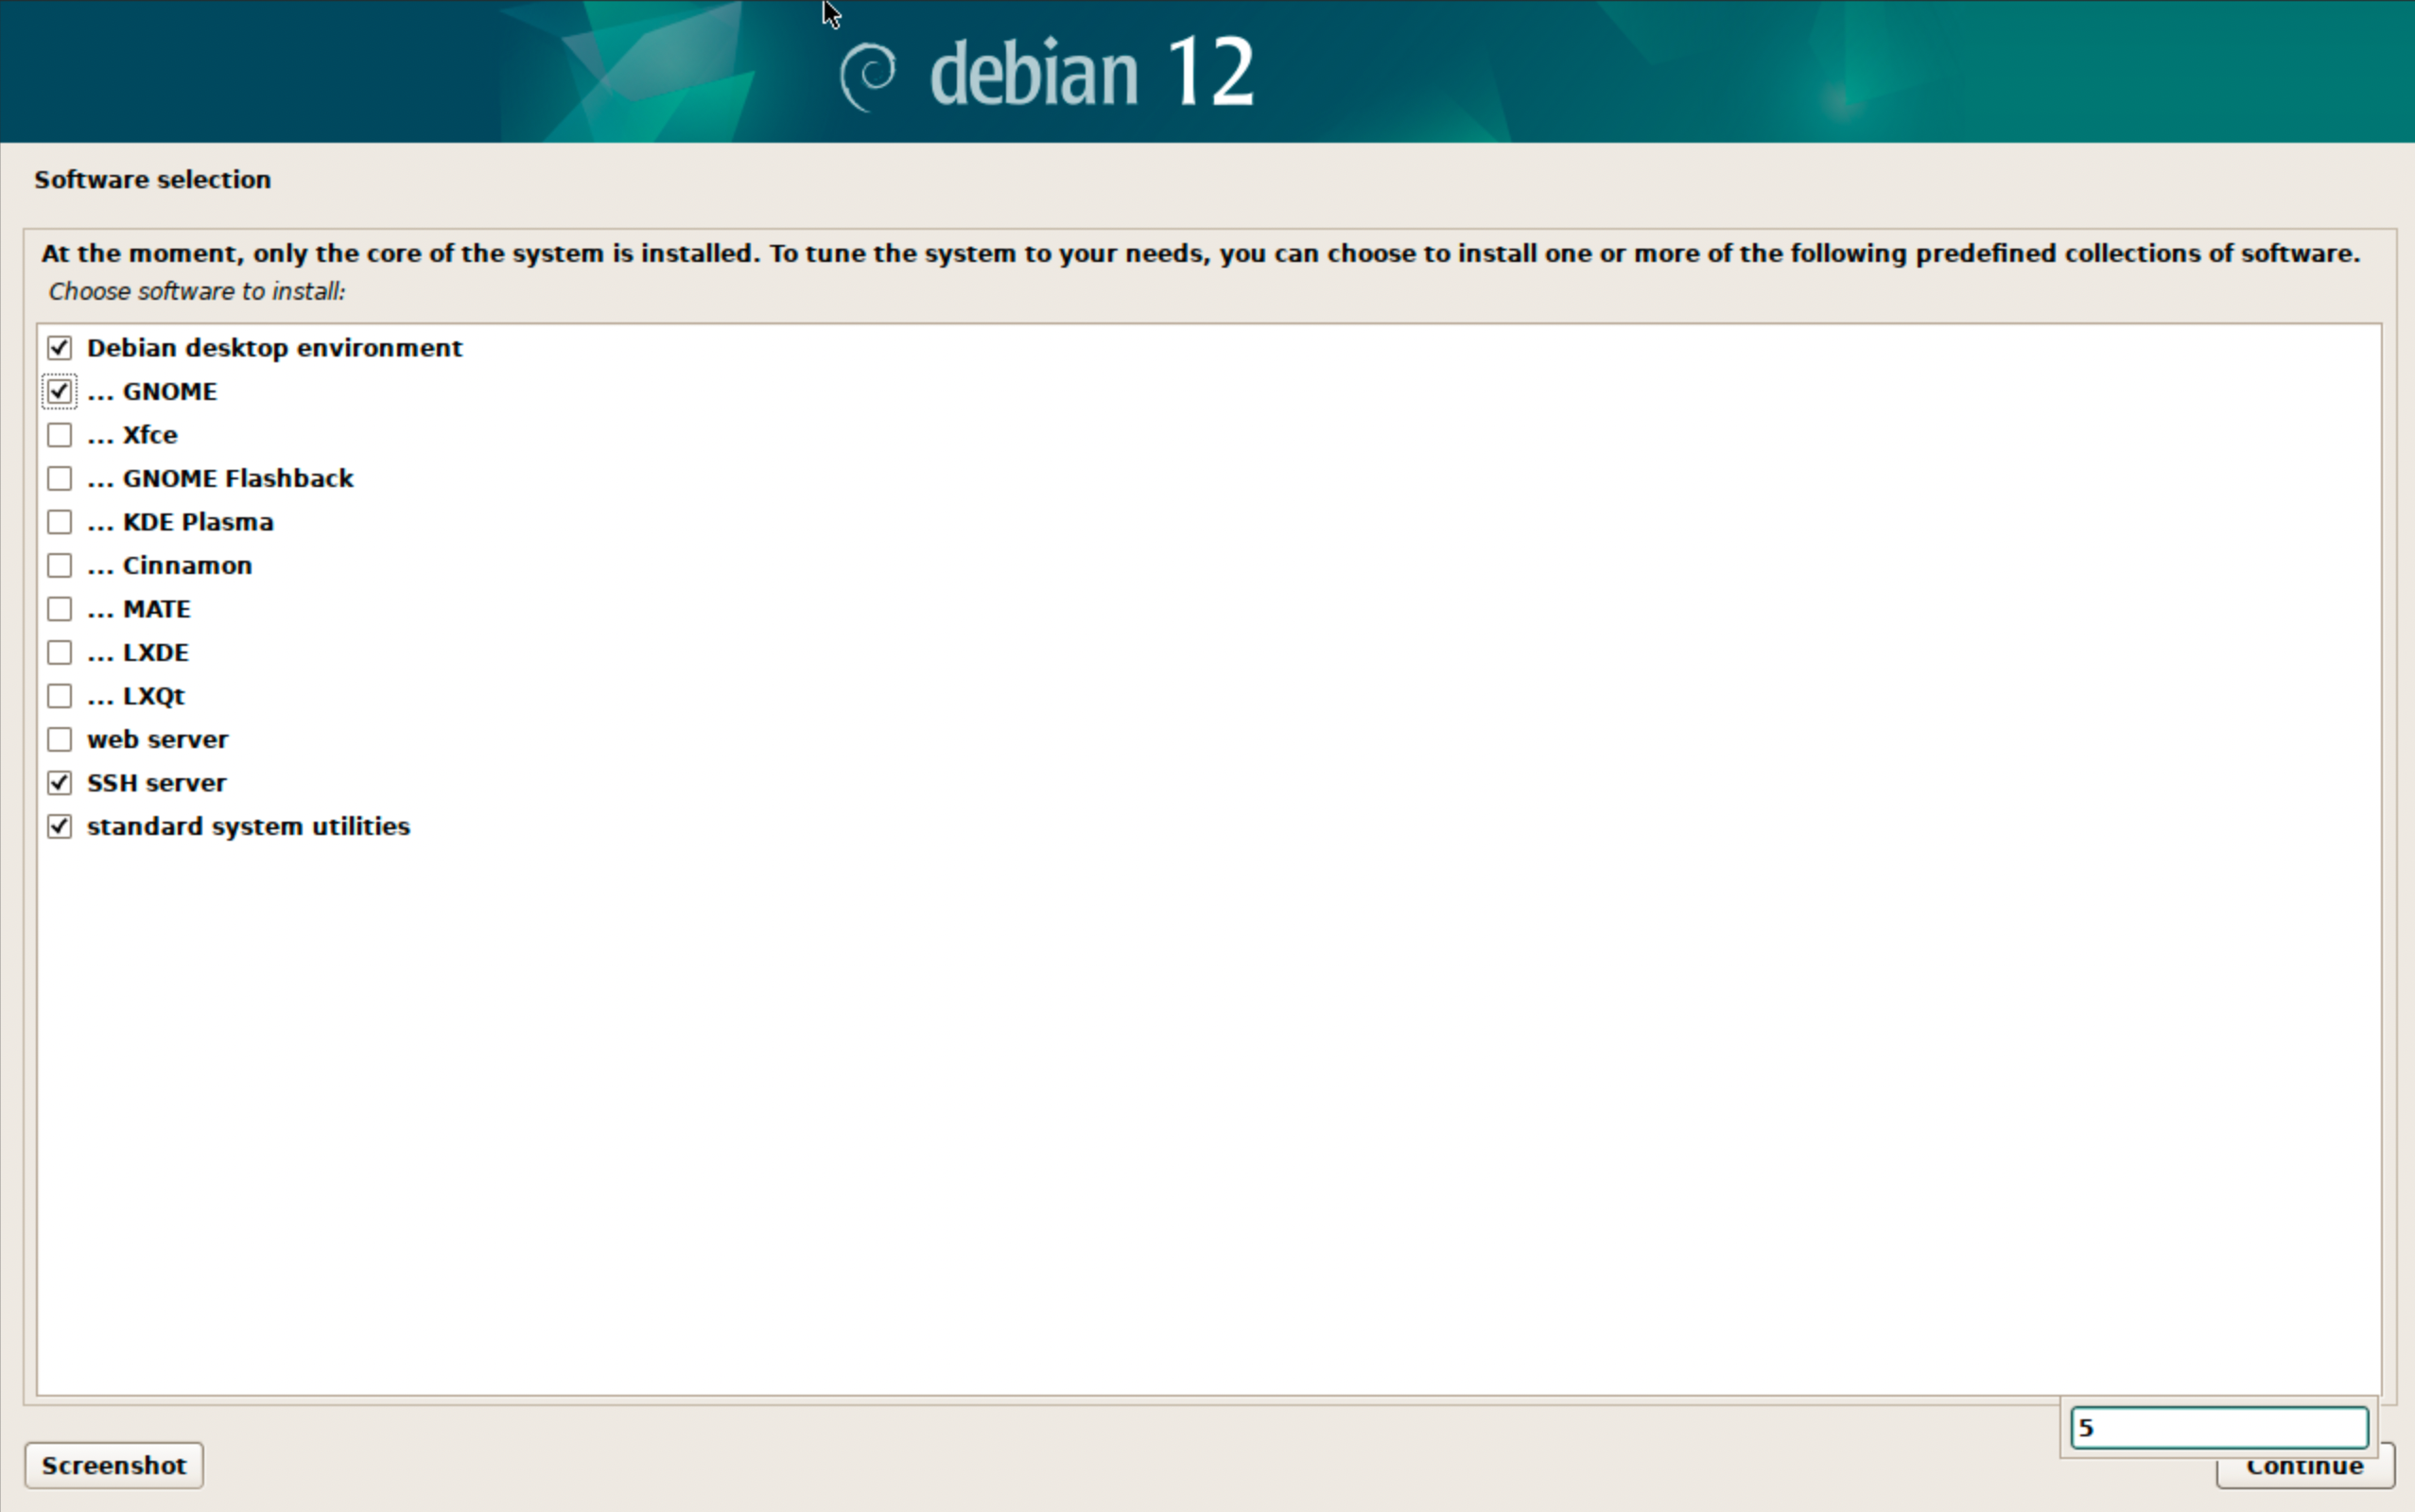
\includegraphics[width=0.7\textwidth]{1-1-1.png}
    \caption{Debian 安裝精靈}
  \end{figure}
  \begin{figure}[H]
    \centering
    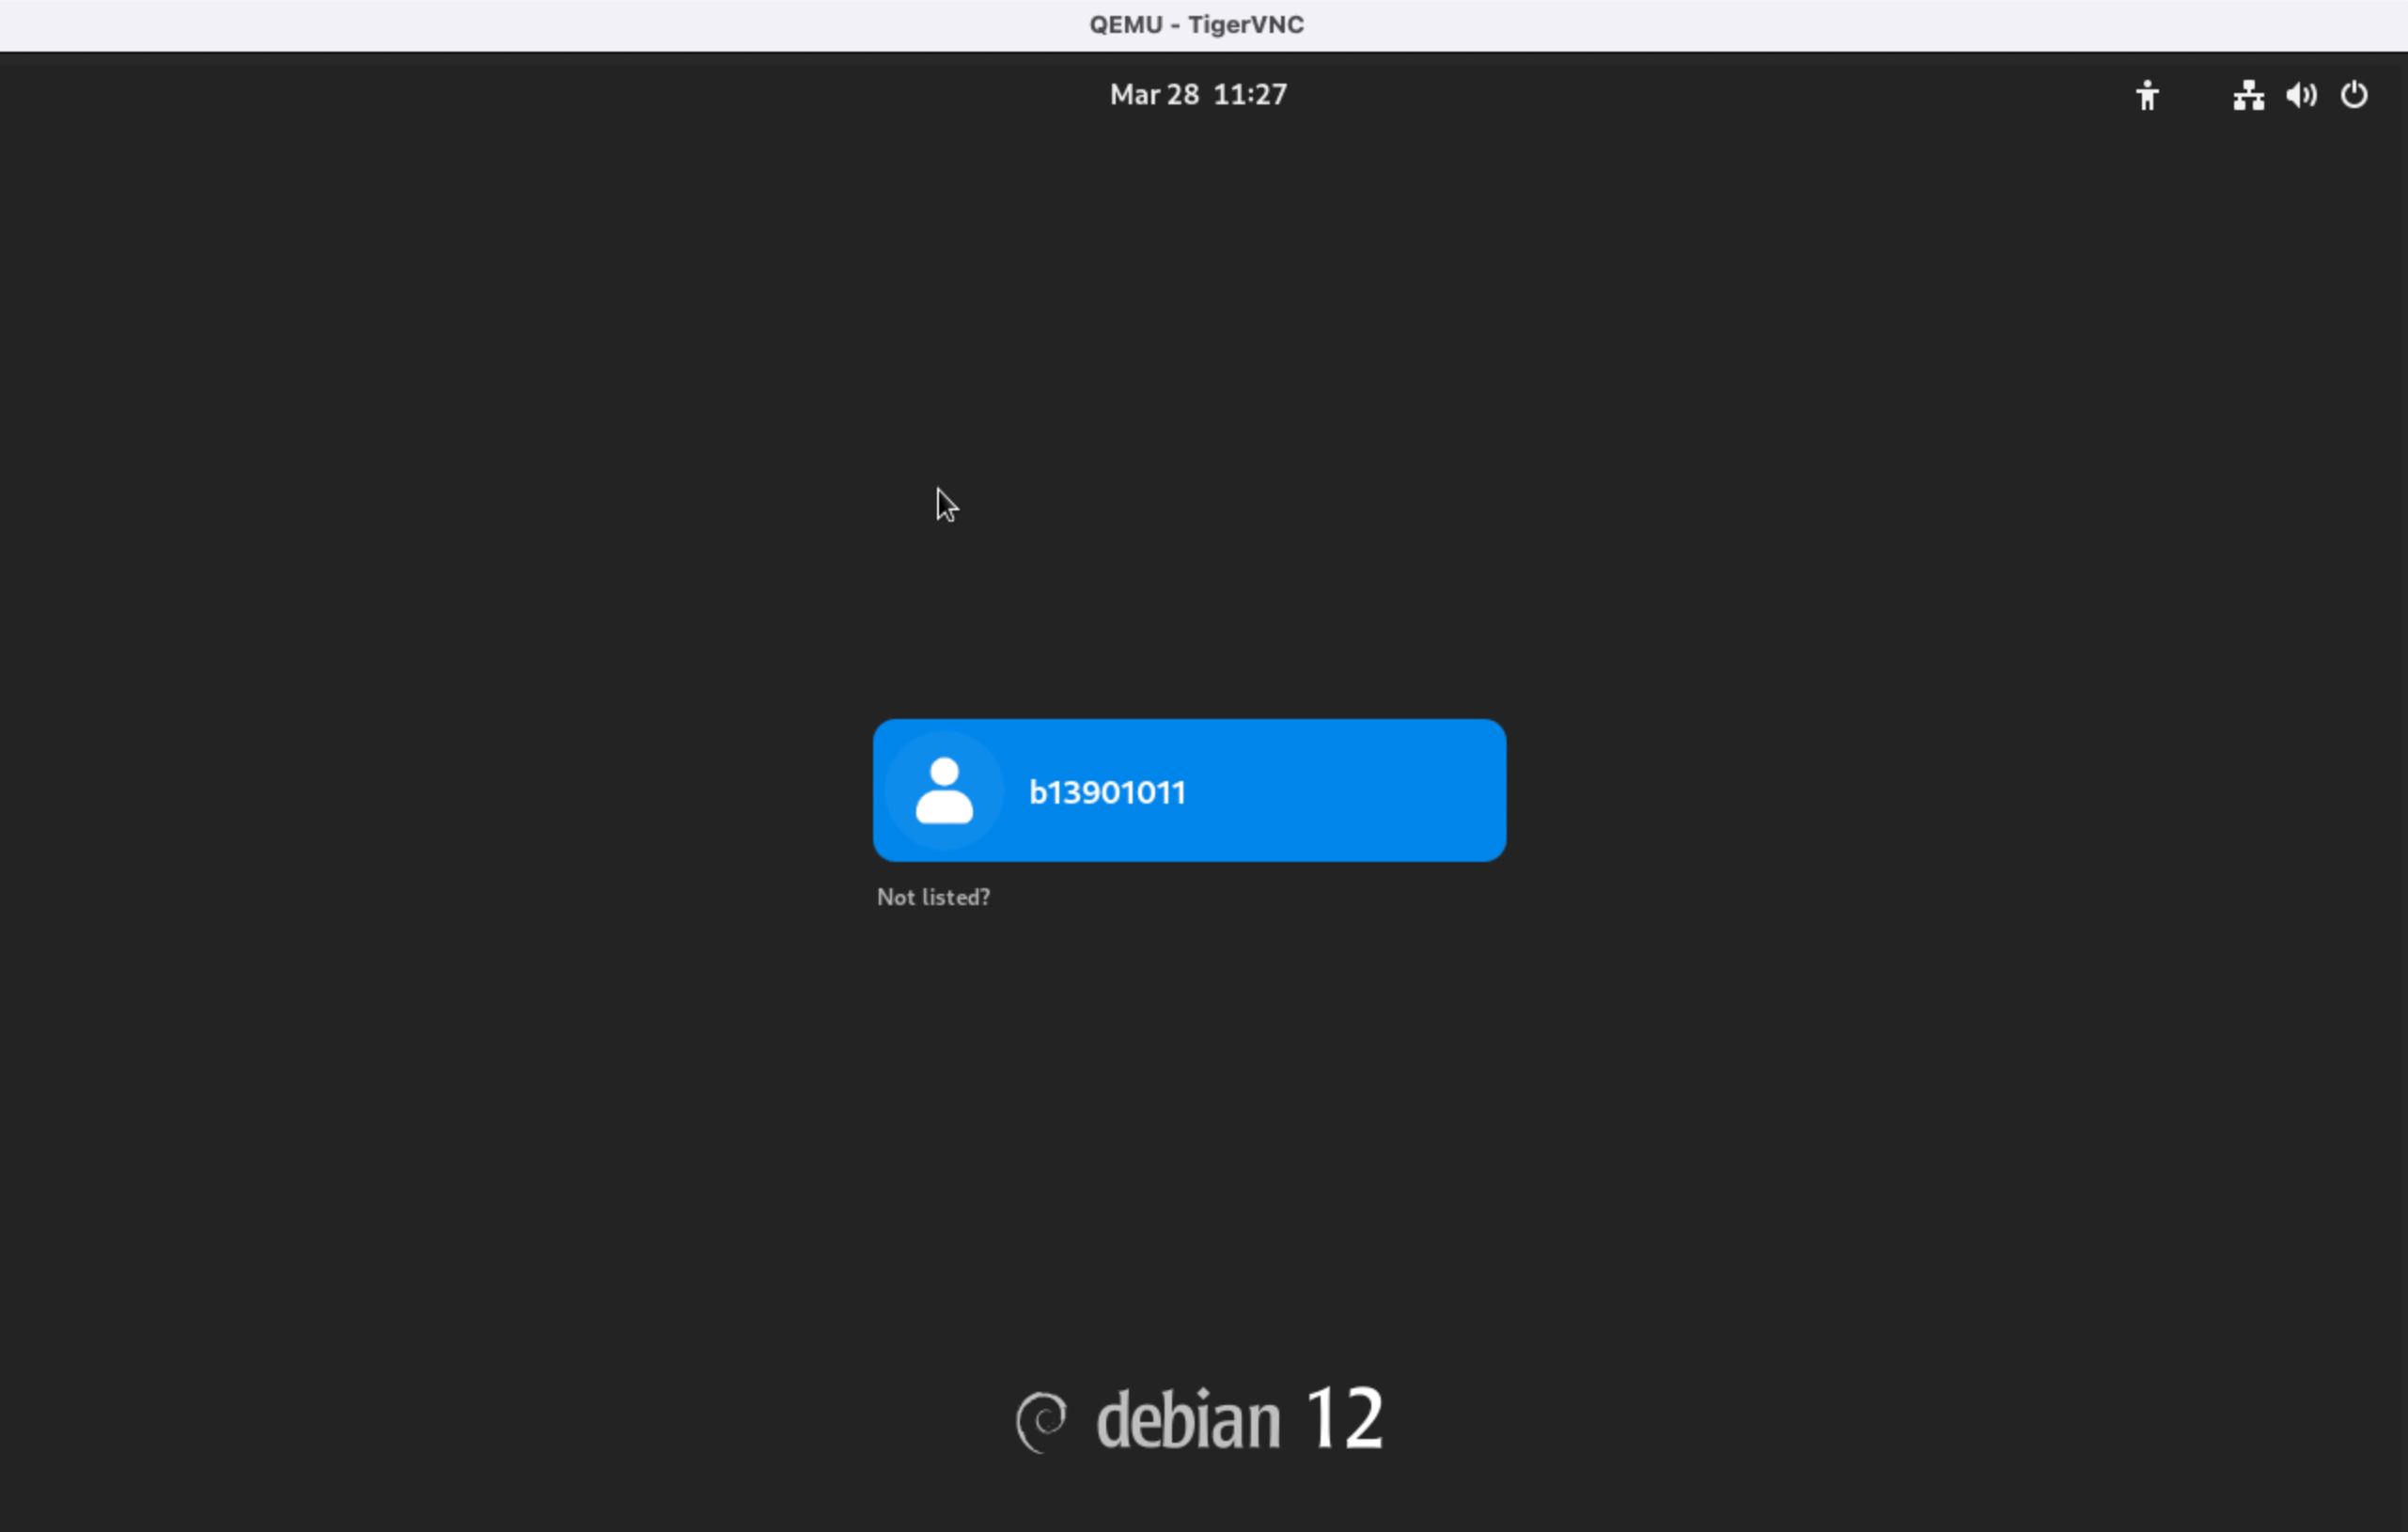
\includegraphics[width=0.7\textwidth]{1-1-2.png}
    \caption{完成 Debian 安裝}
  \end{figure}

  \item 安裝完成後，我關閉虛擬機器，並且參考 Homework 2，建立一份 \texttt{run\_vm.sh} 作為開啟虛擬機器的 Shell Script。這個腳本會開啟虛擬機器，並且將 VNC 連線的 port 設定為 7000，SSH 的 port 設定為 4321。在 \texttt{change vnc password} 之後，就可以透過 VNC 連線到虛擬機器，並且使用 SSH 連線到虛擬機器。
  \begin{minted}{bash}
    #!/bin/bash
    qemu-system-x86_64 \
      -enable-kvm \
      -vnc :1100, password=on \
      -monitor stdio \
      -m 2048 \
      -smp 2 \
      -cpu host \
      -drive file=debian.qcow2 \
      -boot d \
      -net nic -net user,hostfwd=tcp::4321-:22
  \end{minted}
  
  \item 在工作站上，使用 \texttt{ssh b13901011@localhost -p 4321} 連線到虛擬機器，並且輸入 \texttt{su -} 進入 root 權限。
  \item 執行以下指令安裝必要的套件。
  \begin{minted}{bash}
    apt update
    apt upgrade -y
    apt install -y sudo vim git curl wget net-tools libpq-dev neofetch
  \end{minted}
  \item 將我的使用者加入 sudo 群組。
  \begin{minted}{bash}
    usermod -aG sudo b13901011
  \end{minted}
  \item 安裝 MariaDB。
  \begin{minted}{bash}
    sudo apt install mariadb-server mariadb-client
    sudo systemctl start mariadb
    sudo systemctl enable mariadb
  \end{minted}
  \item 以 \texttt{sudo mysql -u root} 登入 MariaDB，並且執行以下指令設定 root 密碼。
  \begin{minted}{sql}
    CREATE DATABASE powerdns;
    GRANT ALL ON powerdns.* TO 'powerdns_user'@'%' IDENTIFIED BY 'b13901011';
    FLUSH PRIVILEGES;
    EXIT;
  \end{minted}
  \item 停止 systemd-resolved 服務
  \begin{minted}{bash}
    sudo systemctl stop systemd-resolved
    sudo systemctl disable systemd-resolved
  \end{minted}
  \item 修改 DNS 設定檔案 \texttt{/etc/resolv.conf} 的內容：
  \begin{minted}{bash}
    sudo unlink /etc/resolv.conf
    sudo vim /etc/resolv.conf
  \end{minted}
  \vspace{-0.5cm}
  \begin{minted}{bash}
    # /etc/resolv.conf
    nameserver 8.8.8.8
    nameserver 8.8.4.4
  \end{minted}
  \item 加上指定版本的 Repository： \\
  修改 \texttt{/etc/apt/sources.list.d/pdns.list} 的內容，新增如下：
  \begin{minted}{bash}
    deb [signed-by=/etc/apt/keyrings/auth-49-pub.asc] http://repo.powerdns.com/debian bookworm-auth-49 main
  \end{minted}
  修改 \texttt{/etc/apt/preferences.d/auth-49} 的內容，新增如下：
  \begin{minted}{bash}
    Package: auth*
    Pin: origin repo.powerdns.com
    Pin-Priority: 600
  \end{minted}
  
  並且安裝 PowerDNS。
  \begin{minted}{bash}
    sudo install -d /etc/apt/keyrings; 
    curl https://repo.powerdns.com/FD380FBB-pub.asc | sudo tee /etc/apt/keyrings/auth-49-pub.asc &&
    sudo apt-get update &&
    sudo apt-get install pdns-server pdns-backend-mysql 
  \end{minted}
  \item Import PowerDNS database schemas to MariaDB
  \begin{minted}{bash}
  mysql -u powerdns_user -p powerdns < /usr/share/pdns-backend-mysql/schema/schema.mysql.sql
  \end{minted}
  \begin{figure}[H]
    \centering
    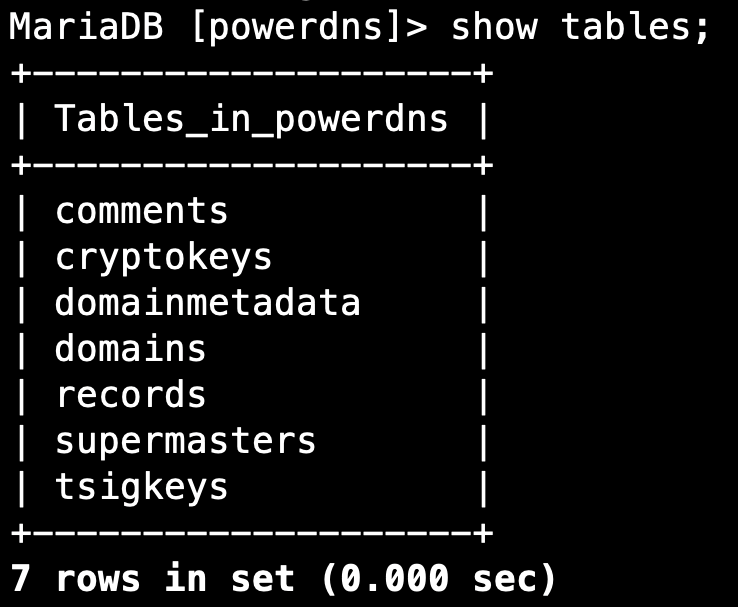
\includegraphics[width=0.5\textwidth]{1-1-3.png}
    \caption{powerdns database schemas}
  \end{figure}
  \item 修改 PowerDNS 設定檔案 \texttt{/etc/powerdns/pdns.conf} 的內容，新增如下：
  \begin{minted}{bash}
    #################################
    # local-port    The port on which we listen
    #
    local-port=5301
  \end{minted}
  \item 新增一個檔案 \texttt{/etc/powerdns/pdns.d/pdns.local.gmysql.conf} 存放 powerdns 的 database 相關設定，內容如下：
  \begin{minted}{bash}
    # MySQL Configuration
    # Launch gmysql backend
    launch+=gmysql
    # gmysql parameters
    gmysql-host=127.0.0.1
    gmysql-port=3306
    gmysql-dbname=powerdns
    gmysql-user=powerdns_user
    gmysql-password=b13901011
    gmysql-dnssec=yes
    # gmysql-socket=
  \end{minted}
  \item 修改設定檔案的權限：
  \begin{minted}{bash}
    sudo chown pdns: /etc/powerdns/pdns.d/pdns.local.gmysql.conf
    sudo chmod 640 /etc/powerdns/pdns.d/pdns.local.gmysql.conf
  \end{minted}
  \item 測試 PowerDNS 是否能正常運作：
  \begin{minted}{bash}
    sudo systemctl stop pdns.service
    sudo pdns_server --daemon=no --guardian=no --loglevel=9
  \end{minted}
  \vspace{-0.3cm}
  \begin{figure}[H]
    \centering
    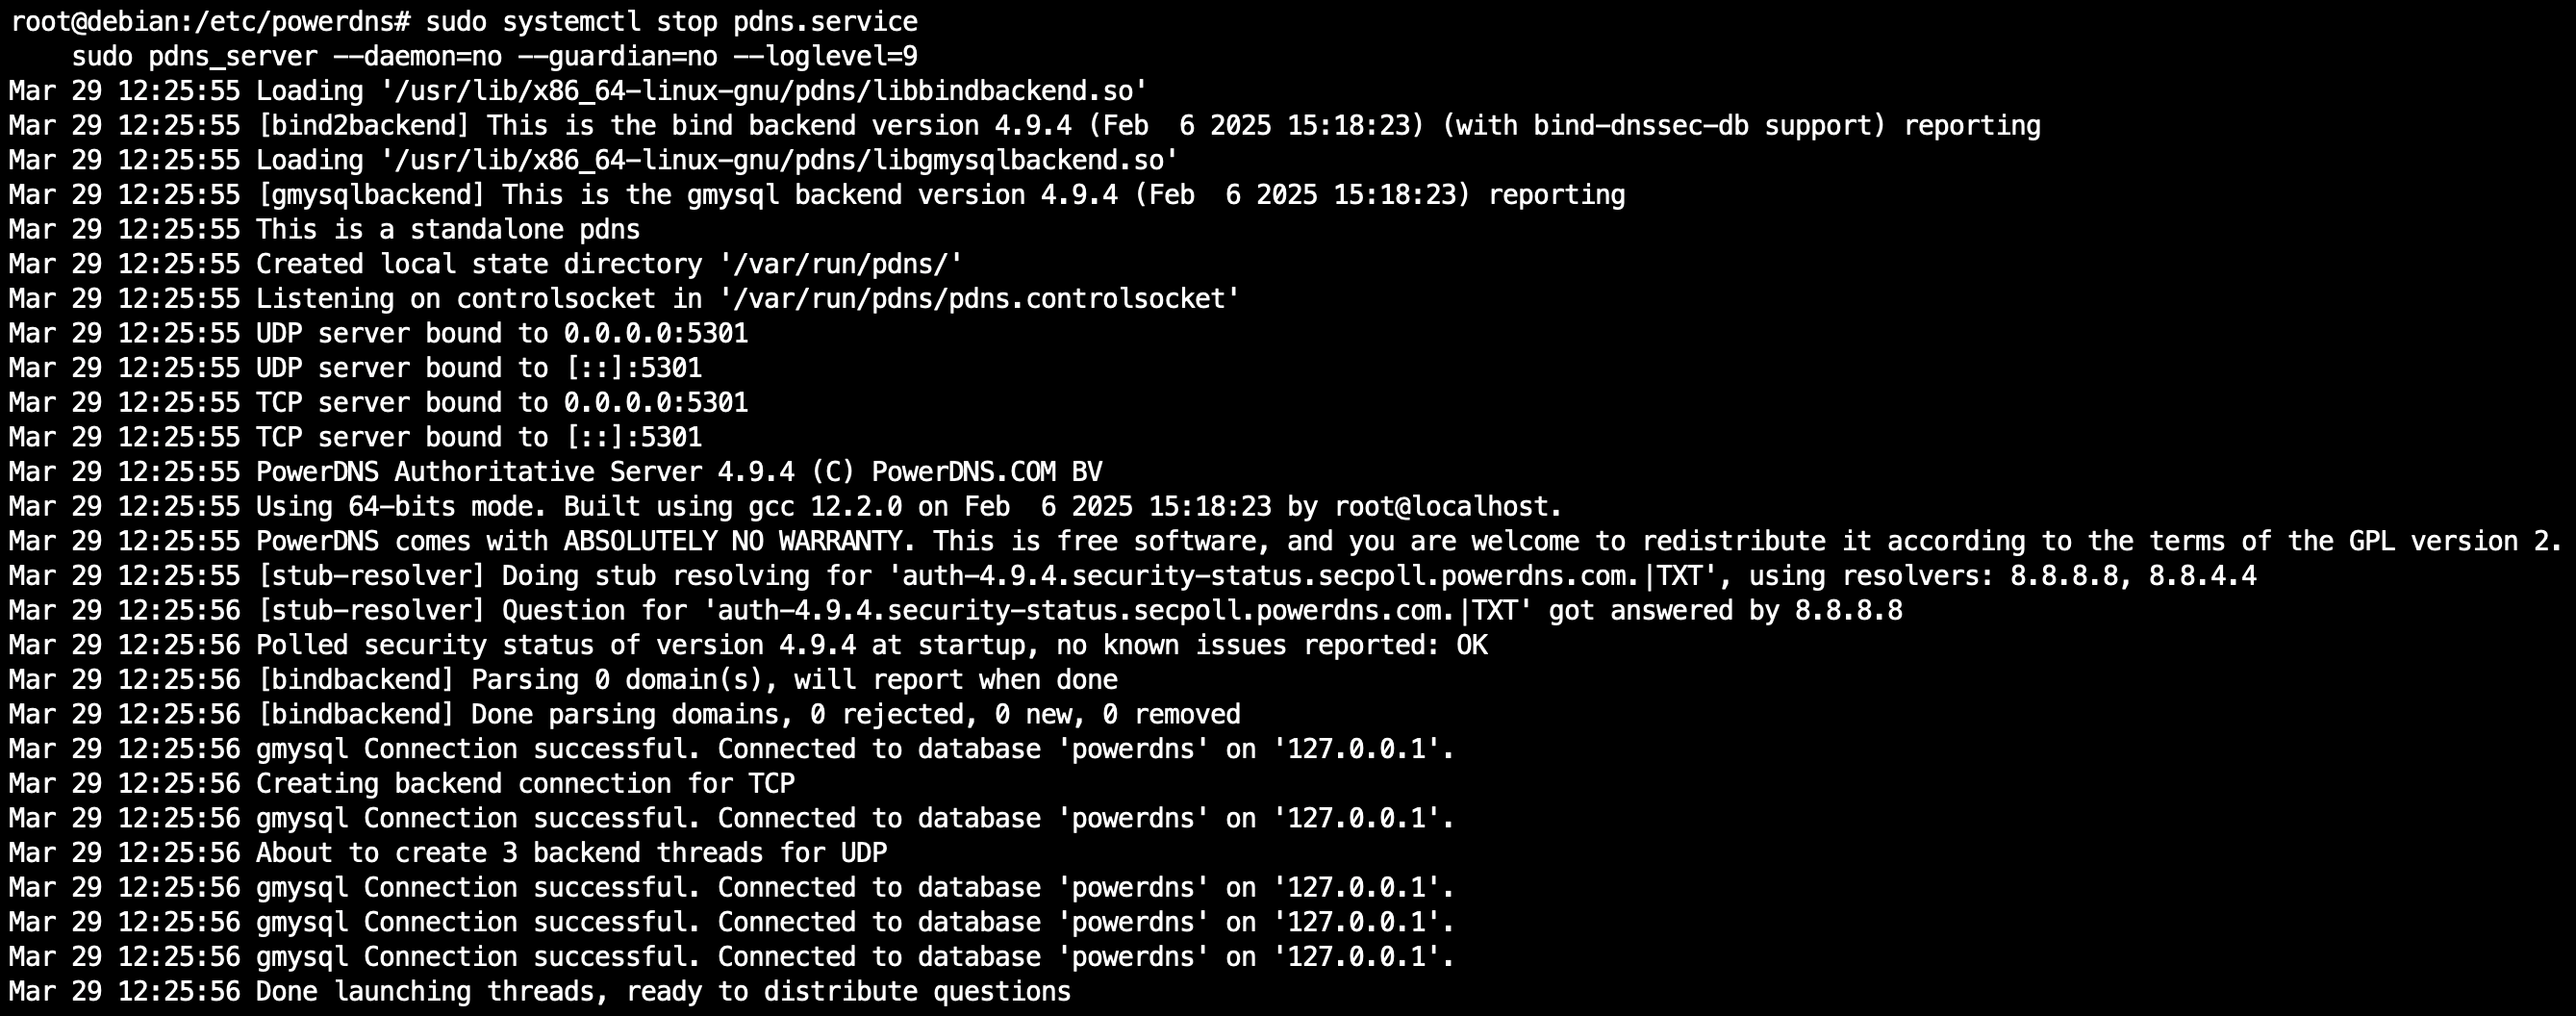
\includegraphics[width=\textwidth]{1-1-4.png}
    \caption{PowerDNS 測試}
  \end{figure}
  \item 確認沒問題後，重新啟動 PowerDNS 服務，並且截圖題目要求的畫面。
  \begin{minted}{bash}
    sudo systemctl restart pdns
    sudo systemctl enable pdns
  \end{minted}
  \begin{mycolorbox}[green]
    \textbf{Answer:} \\
    \vspace{-1cm}
    \begin{figure}[H]
      \centering
      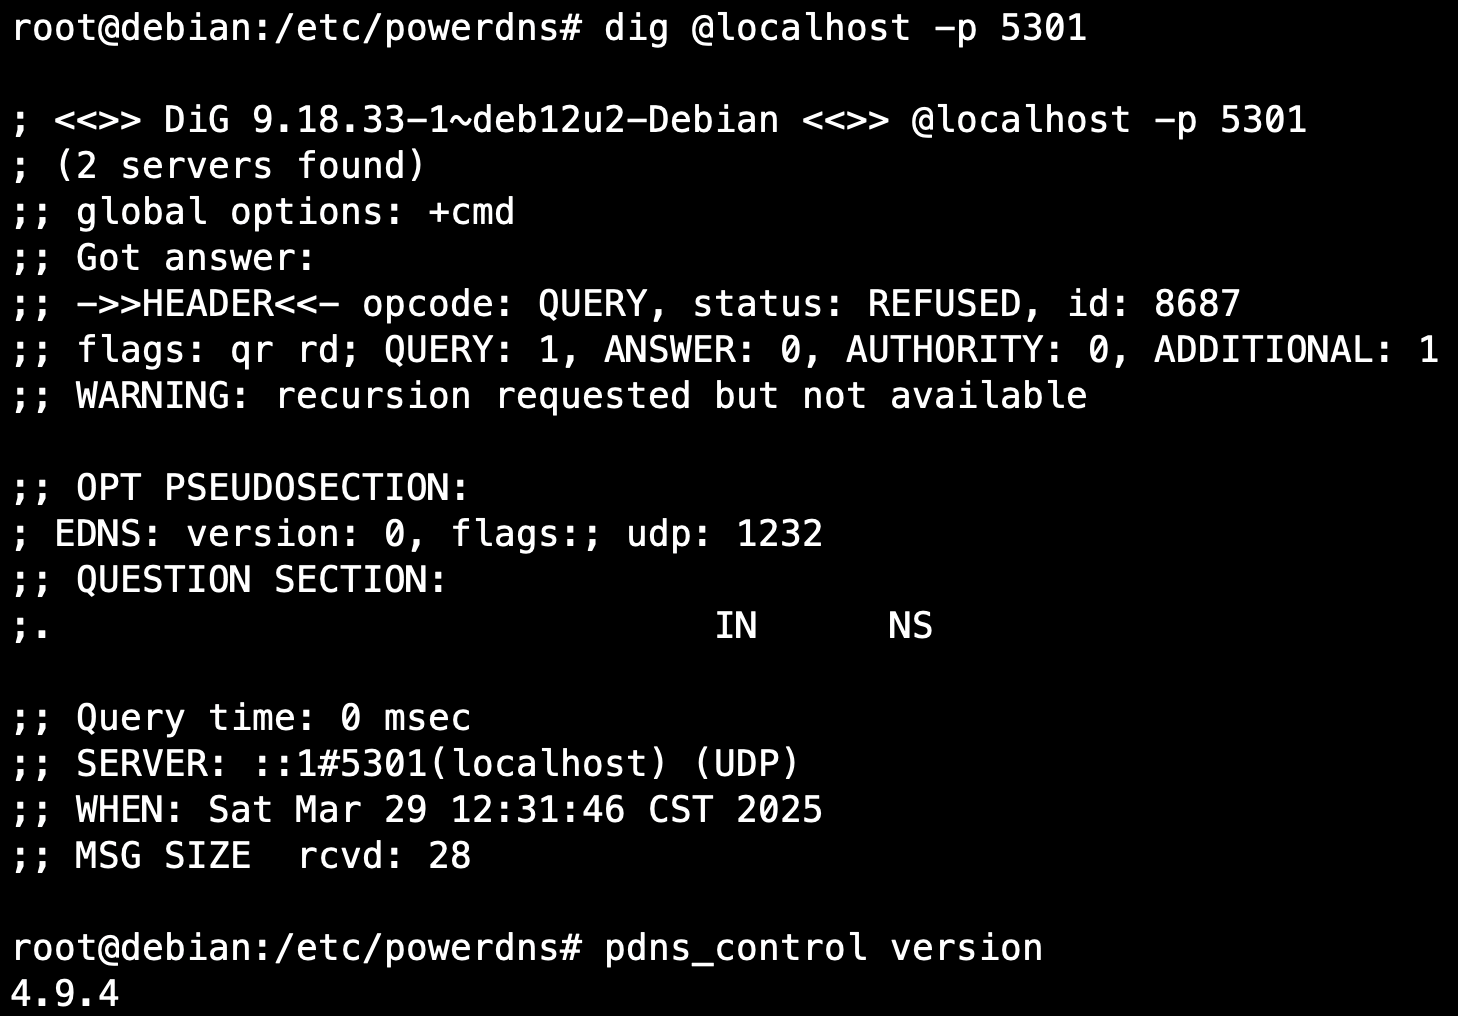
\includegraphics[width=0.69\textwidth]{1-1-5.png}
      \caption{\texttt{dig @localhost -p 5301} 以及 \texttt{pdns\_control version} 結果}
    \end{figure}
  \end{mycolorbox}
\end{enumerate}




% -----------------------------------------------------------
%    You don't have to mess with anything below this line.
% -----------------------------------------------------------

\end{document}
